\chapter{What is LDAP}
Before starting to create the deception component generator, it's usefull to understand what LDAP is.
\\\\
LDAP stands for Lightweight Directory Access Protocol, so it’s a protocol to make queries and modify a directory service.  
\\
In fact, the protocol does not include a directory service per se, but some implementations of it also have an integrated directory service. 
\\
At the beginning, the LDAP protocol was conceived to create an alternative for the DAP protocol, in particular a less resource intensive and lighter one. LDAP was also conceived to use the TCP/IP protocol to make operation related to the X.500 directory easier.  
\\\\
The LDAP protocol has been updated over the years and now it’s at the third version. 
\\
In the third version of the protocol, the simple authentication and security layer (SASL) was added, which is a framework for authentication and security in the internet protocols. 
\\\\
\section{How it works}
As previously mentioned, the directory could be a generic one, that is possible thanks to the interface, called DataBase Interface easily implementable in a module to guide the beckend. 
\\
The DBI manages a collection of entry or objects. The entries are a composed by attributes, which have a type and one or more values. Every entry has a Distinguish name (DN), that also indicate the position from the root.
\\
The entries are also hierarchically ordered, and the final structure is called DIT (Directory Information Tree) and is a way to store the representation of the DB managed by the DBI.
\begin{figure}[h]
    \caption{How LDAP works}
    \centering
    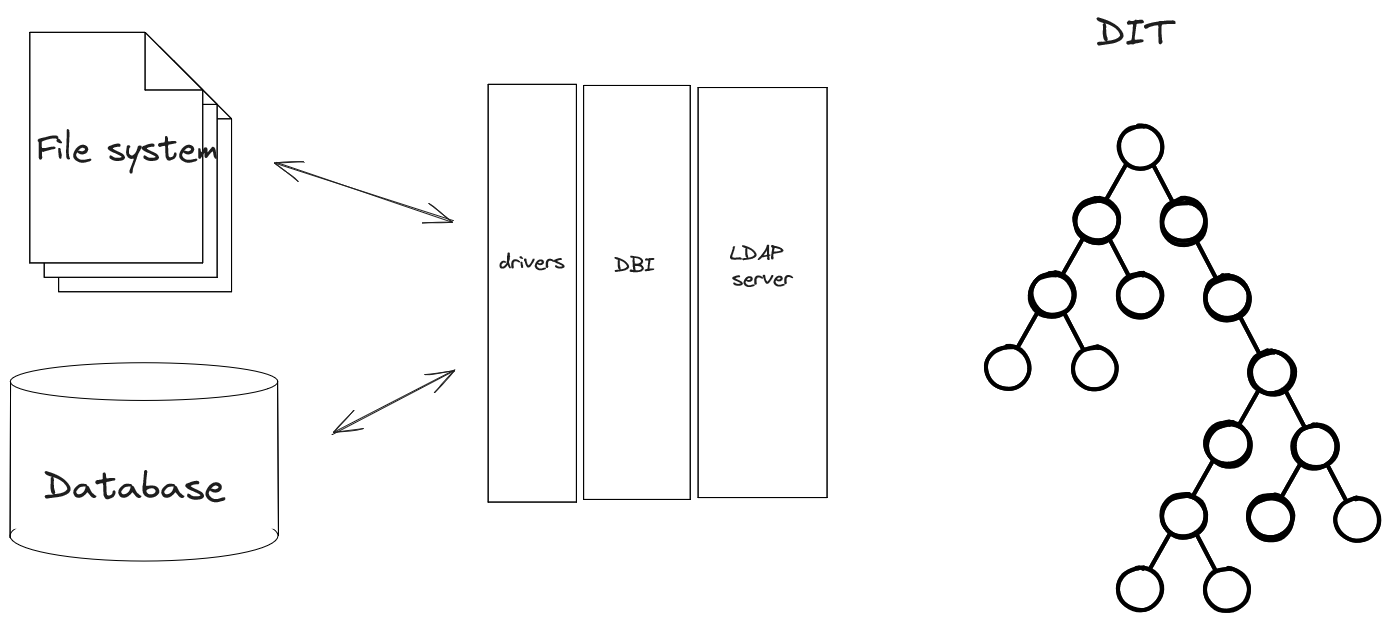
\includegraphics[width=\textwidth]{img/arch.png}
\end{figure}
\\
It is used a hierarchy because LDAP was born as a system to organize data about people and resources inside a company. The hierarchy also allows us to make direct links to the data, an easy partitioning system to administrate, control the access and locate easily data. 
\\\\
An entry is a collection of the attributes, in which the value of it is stored directly, and it’s labeled by the type of itself.
\\
Between the various possible attributes, two must be indicated: dn and one or mode objectClass. This format is also used to exchange entries between client and server, and is called LDIF (LDAP interchange format). 
\\
For inserting an entry it’s necessary to have well formatted objects and a uniform view of the data, commonly used between all the users. This is the function of a SCHEMA. A schema is a set of rules that describes the data and have two types of definitions: 
\begin{itemize}
    \item ObjectClass 
    \item attributeType 
\end{itemize}
\\
Every entry is based on one or more objectClass, which describes the types of attributes that must or should be in the entry.  Every attribute has its own type, with also the set of rules necessary to compare them. 
\\
The attribute type can be one of the commonly used or can also be described by the user, but in that case, it must be defined in a file and added to the server configuration. It can be done using the ldif format or a schema file.
\\
This is valid also for objectClass.
\begin{mdframed}[backgroundcolor=back1]
    \begin{lstlisting}[style=bash, caption={Example of definition of an attributeType (for objectClasses is similar)}]
olcAttributeTypes: (...)
    DESC 'name'
    EQUALITY caseMatch
    SUBSTR caseMatchSubs
    SYNTAX ....
    \end{lstlisting}
\end{mdframed}
\begin{figure}[h]
    \caption{Correspondance between schema definition and DIT elements}
    \centering
    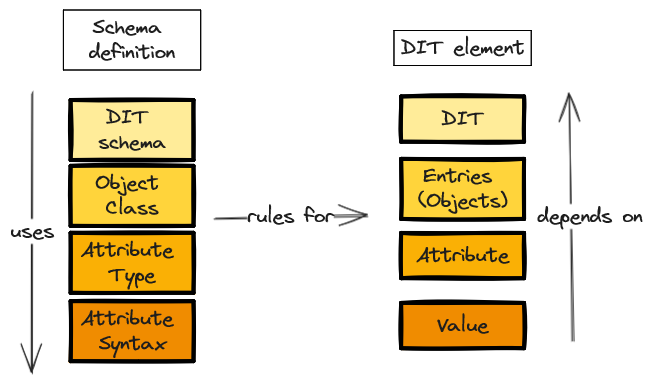
\includegraphics[width=\textwidth]{img/dit.png}
\end{figure}
\\\\
One famous implementation of LDAP is OpenLDAP, which includes the Access protocol and a directory. This is the one choosen to create the docker image to configure.
%% TODO: insert OpenLdap logo
